\TBD{This section gives general description of reconstruction and
  calibration:
\begin{itemize}
\item Definitions of Calibration Interval (\CI) and Update Interval (\TI)
\item State why kind of data is calibrated/reconstructed in FLP's
  (clusters, masks ets) and what on EPNs
\item How the calibration from FLP propagates to EPNs and from FLP and
  EPN's to OCDB. 
\item Treatment of \TF edges in calibration and reconstruction
\item Preferences for the \TF duration (variable, fixed)
\item Calibration feedback loop ("predictive step").
\item Outline of reconstruction flow, detector dependencies.
\item Alternatives: full reconstruction at once vs partial
  reconstruction (e.g. high \pt tracks) for calibration ("cpass") followed by
  full reconstruction.
\end{itemize}
}

One of the main challenges for ALICE at \run{3} is without doubt the extremely high data taking rates that will 
bring the experiment to receive data with a speed 2 orders of magnitude higher than at \run{1}, 
jumping from 500 Hz to 50 kHz. The physics motivations for this were well described in~\ref{upgradeLOI}. Here,
the necessity to perform online calibration and reconstruction was also presented, with the main aim at 
reducing the data volume to an affordable size for permanent storage. 

The highest data reduction factor which
is expected is $\sim 20$, coming from the TPC detector which will be read out in continuous mode at \run{3} leading
otherwise to unaffordable data storage.
It is clear that to achieve such factors, zero suppression techniques and coding algorithms won't be enough, and 
a substantial part of the data reduction will be reached only through reconstruction of tracks discarding the data
that do not carry physics information (e.g. clusters from
$\delta$-rays, unreconstructable tracks etc.). 

The strong coupling between calibration and reconstruction that was effectively demonstrated during \run{1} will 
be complicated by the extreme conditions in terms of luminosity that will characterize \run{3} data taking. Time
dependence of calibration will become even more pronounced, and the statistics requirements of calibration 
will have to deal with the new data flow that will accommodate both continuous and triggered read out.  

In order to understand the calibration and reconstruction data flow, it is important to summarize a few concepts.
\begin{itemize}
	\item \textit{Time Frame (TF)}: data will be sent from the FLPs to the EPNs after being aggregated in blocks where multiple
	events will be present at the same time, in order to combine the data from detectors read in triggered and 
	continuous mode; the boundaries of the time frames will be defined by a heartbeat triggered received by all detectors. The
	foreseen duration of the TF will be $\sim 100$ times the drift time inside the TPC detector. The possibility to 
	have an adjustable TF duration which counterbalance the decrease in luminosity in time in order to level the 
	statistics contained in one TF is under discussion. Both scenarios (namely, fixed and varying TF duration) have to 
	be considered when defining the calibration and reconstruction data flow.
	\item \textit{Calibration Interval (CI)}: \textcolor{red}{I am not sure whether this is important...} since calibration is strongly
	related to the data taking conditions, a CI can be defined as a period where stability is guaranteed. This could refer 
	to detector configuration, beam conditions... 
	\item \textit{Update Interval (UI)}: time-dependent calibrations require an update of the relevant calibration parameters
	with a frequency that strongly depends on the calibration itself (and as such, on the detector and its requirements). A UI 
	corresponds to the time between the moment when calibration data start to be collected, and the last moment when they
	are used. In terms of data taking this corresponds to a period during which a detector can be considered stable. 
	\item \textit{Feedback Loop (FL)}: the interdependency of calibration and reconstruction that was fully demonstrated during 
	\run{1} implies that calibrations that are produced during reconstruction should be then used for the reconstruction 
	of the next data. The FL is the concepts that describes this dependency.
\end{itemize} 

\subsection{Processing in FLPs}
\label{sec:Processing in FLPs}
The first layer of data processing will be the FLP. Here, the data will come from the detectors through DDL links and 
RORC3 cards. RORC3 cards will be equipped \textcolor{red}{(I guess)} with FPGA cards, where cluster finding will be 
possible as it was done during \run{1} for the TPC. When shipped to the FLPs' memory, further data processing will 
be possible, exploiting possible GPUs on 
the machines. The single FLP is foreseen to be connected to a maximum
of 12 optical links, while for instance, the TPC will be served by
1836 DDLs.
. \textcolor{red}{It is not
clear to me whether, in case a detector has only one DDL, it will be connected to the same FLP as another detector, but
I assume not. In any case, I don't foreseen any cross-talk between
different detector's data.}. 
This, obviously, limits the amount of 
data that can be processed in an FLP per detector, and as a consequence rules out at this stage any processing that
relies on the whole detector's data and/or on data from different detectors. Procedures such as cluster finding will 
be limited to the part of detector connected to the FLP. As a result, the same physical cluster could be found on two 
different FLPs. The way this doubled information will be treated in the EPNs will be detector specific, and could imply
merging of clusters, or discarding of one of the two. 

It is important to mention here that FLPs will receive all the data from the detector part they are connected to. Despite the
limit in ``detector slice'' it is processing that it
% will occur at this stage 
will 
%then 
benefit from having at its disposal all the statistics. 

As already mentioned, data will come to the detectors with a rate of 50 kHz, with a peak input to the FLPs of 1 TByte/s. 
Assuming 250 FLPs in the online farm (following the current estimates from the O$^2$ project), each FLP will receive
4 GByte/s. With a tentative hypothesis of 20 GBytes of memory in each FLP dedicated to data processing, and bearing in 
mind that part of the resources will be used for data transport, one could conclude that a processing rate of 2 s/GByte
could be reasonable. Nevertheless, the data will have to be exported to the second layer of processing with the same 
frequency with which they arrived on the FLPs, in order to not create data traffic jam over the network. 

\subsection{Processing in EPNs}
\label{sec:Processing in EPNs}
From the FLPs, data are aggregated in time frames, and then sent to EPNs. The length of a TF will be of the order of
$100 \div 1000$ times the drift time in the volume of the TPC ($\sim 100 \mu s$), which means $10 \div 100$ ms. Whether such
duration will be fixed or variable is currently under discussion. For simplicity we will assume here that it is fixed to 
$100$ ms. 

While on the FLPs data are split per detector and per detector ``slices', on the EPNs they will be merged together. 
This is an important difference with respect to EPNs, since interconnections between detectors will be possible at this 
stage. On top of containing the data read-out by the detectors, the TF will also transport from the FLPs the calibration
information that was produced there (if any, and as soon as they are available). Due to the processing rate of the FLPs,
and to possible statistics requirements for calibrations, it could happen that some calibrations are ready to be sent 
the the EPNs only after a certain amount of time frames have been collected and prepared. \textcolor{red}{It is to be evaluated 
whether such cases exist, how much statistics they would need, and then one should combine it with the possibility
that TF are sent not one-by-one, but in groups of many (as presented at the O$^2$ meeting in January). If the second
option is implemented, maybe there is time to prepare the calibrations before sending the data to EPNs.} The calibration
data size is expected to be smaller and negligible compared to the detector data size.

On top of receiving the data from the detectors, the EPNs will also 
receive data from
%be connected to 
the Detector Control System (DCS
\textcolor{red}{at least I hope}), which will add to the time frame \textcolor{red}{(I don't know if embedded
in the data or not)} detector specific information such as configurations, temperatures and high voltages. The DCS 
information could be used as input for calibrations in the EPNs. 

The EPNs will be the natural place to perform the first steps of the 
%reconstruction
tracking. Due to the fact that only a course
calibration is possible at this stage, the primary goal of this reconstruction should be data reduction. For this reason, 
mainly detector standalone procedures are expected to occur at this stage, such as ITS track finding and fitting, 
vertexing, TPC track finding, and only limited to those steps for which a first level calibration is enough. 

In case tracking is needed for the calibrations to be used at this point, it is important to bear in mind that the data flow in 
terms of time frames imposes some limitations, together with the fact that each EPN is independent from the 
others, and that no information can be exchanged (at this stage) between the EPNs. The distribution of the TF over 
the different EPNs in ``round-robin'', for example, implies that each
EPN will receive (in average) a second time frame only after a 
time equal to the duration of a time frame multiplied by the number of EPNs, i.e., assuming 1500 EPNs, and a TF duration 
of 100 ms, after 2.5 minutes. If some calibrations should occur in the EPNs needing a statistics that can be collected over a 
time which is of the same order as the TF duration, they will then be available only for the subsequent time frame. This 
is possible only if the UI of a calibration is long enough to ensure the stability of the calibration over this time. Even more
complicated is the case when more than one TF is needed to collect the statistics for calibration. The time to be waited
before a calibration can be used would then stretch over several minutes. It is necessary to evaluate which calibration
procedures needed at this first reconstruction step would be affected by this. 

On the other hand, calibrations that take as input only a very limited amount of data collected over a time which is much
smaller than the TF duration could be produced with the first data of the TF, and then used in the reconstruction of the
remaining portion of TF. Depending on the validity of such calibrations, it could be that as soon as a calibration object 
is produced, it is used over several TFs on the same EPN. 

Due to the fact that the EPNs receive the data from all detectors corresponding to the same time frame, in case the 
calibration of one detector depends on the reconstructed data of another one, the reconstruction flow will have to 
follow this requirement \textcolor{red}{(an example is TPC that needs event and track multiplicity information from FIT)}.
Never the less, whenever the calibration of one detector (let's say detector B) depends on the calibration of another
(let's say detector A), a more sophisticated
procedure will have to be adopted. In the assumption that no circular dependency is there between two detectors, 
and that both detectors need to calibrate a fraction of data that is much smaller that the TF duration, one possible 
solution is to start reconstructing, produce with the first data the calibration of detector A, make it available for 
the reconstruction of the rest of the data, and produce the calibration for detector B. This approach implies the 
possibility to produce and use a calibration during the reconstruction of the same TF. An analogous implementation
could be realized in case for the calibration of detector A and B a whole TF is needed, baring in mind the delay
between two TFs on the same EPNs. These considerations make it clear the importance of determining 
inter-detector dependencies.

\subsection{Processing after data reduction}
\label{sec:Processing after data reduction}
In the following, the data flow will be split into steps, as shown in Figure~\ref{fig:Flow}. 

\subsubsection{Step 1}
\label{sec:Step 1}
As it was already discussed, 
clusterization and first 
calibrations are supposed to happen at the beginning of the processing. As soon as the data are assembled in 
one time frame, this is shipped to one EPN. Here, the first algorithms that will be run will be most likely standalone
procedures aimed at data reduction. EPNs should also be able to receive data from DCS. To be noted that at the
very beginning of the fill only the calibrations from the previous fill will be available. As a consequence, in case the 
standalone processing will need calibration from FLPs, either some delay is introduced between FLPs and EPNs
in order to prepare such calibrations, or the first data shipped to the EPNs will not be processed here with the most 
recent calibrations. In the latter case, it could be envisaged, though, a second processing of these data to recover 
them.

The calibrations that are produced at this stage of the processing will be available during the same stage only for the 
data that will come to the same EPNs. This means that up to data compression no cross-talk is foreseen between the
different EPNs. This should be possible since up to this moment no calibrations requiring large fraction of the statistics
seem to be needed. Never the less, EPNs should be able to read from an OCDB-equivalent calibration database 
in order to make use of the calibrations produced in previously standalone runs (e.g. PEDESTAL, NOISE... runs). The 
drawback of such approach is that in case data compression requires some calibrations from the standalone reconstructions,
the first portion of data on each EPN will not be calibrated at first, and a second processing over them will be needed
to recuperate them. The feasibility of such implementation depends on the same argumentations mentioned in 
Sec.~\ref{sec:Processing in EPNs} concerning calibration validity. 

\begin{figure}[htp!]
  \begin{center}
    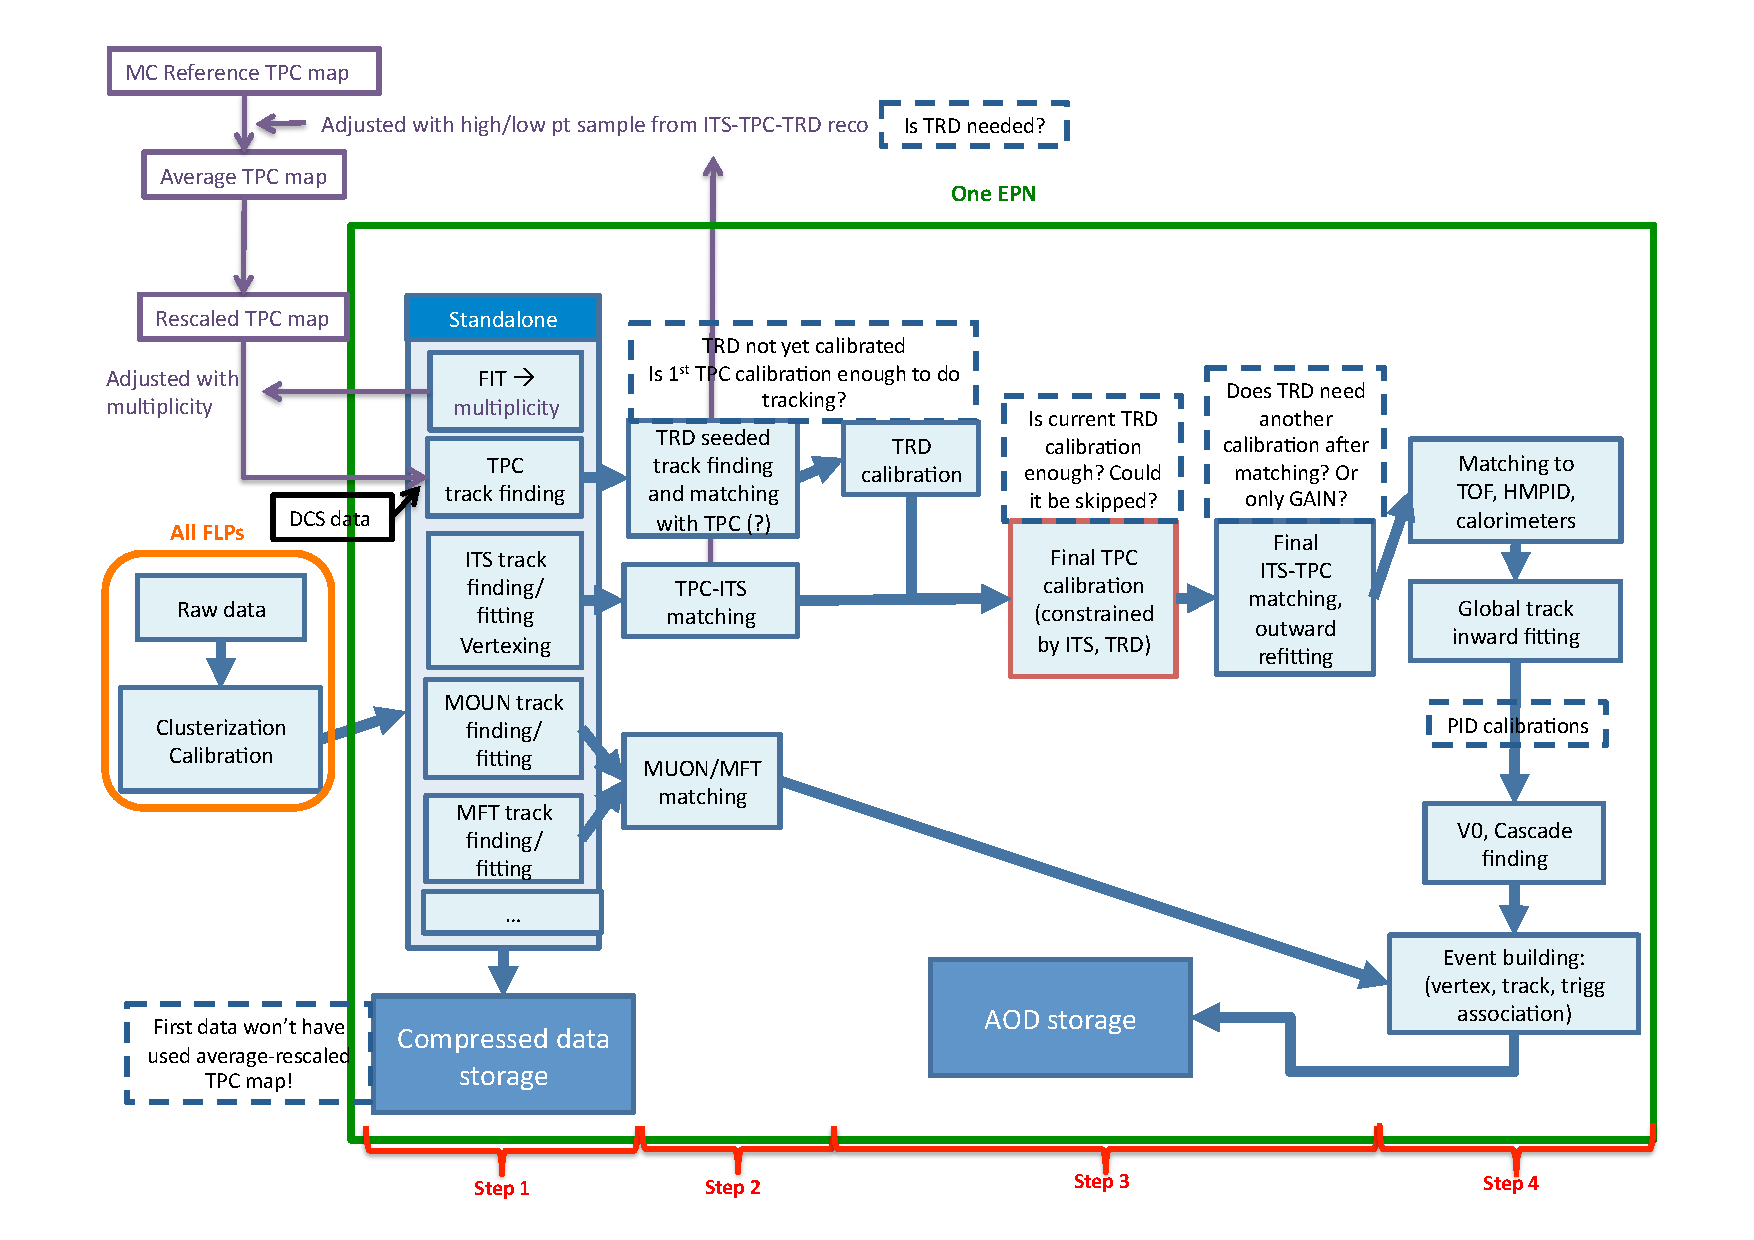
\includegraphics[height=0.67\textheight, angle =90]{general/flow_scenarios.pdf}
    \caption{Schematic
      outline of the reconstruction and calibration data flow.}
    \label{fig:Flow}
  \end{center}
\end{figure}

\subsubsection{Step 2}
\label{sec:Step 2}
The data flow continues from this point with the first inter-detector matching, and tracking stages that could not be performed
before due to missing calibrations. 
% RS: supress?
These processes would still happen on time frame base, on the EPNs. 
%
For example, a first ITS-TPC matching could be performed, and the TRD tracking seeding
using TPC information could take place. \textcolor{red}{Supposing that the TPC output from the EPN is at this point
calibrated enough, TRD could perform its own calibration using tracks, so they would need to match with TPC. For the 
TRD calibration, the same argumentations as in Sec.~\ref{sec:Processing in EPNs} in order to obtain and use the
calibration information on the EPNs.
Moreover, at this step,
a high and low \pt sample could be extracted from the ITS-TPC (also TRD?) matching to provide the rescaling factor 
for the Space-Charge Monte Carlo reference map to be adjusted to the current data taking. Independently from where 
everything is happening online or offline after data reduction, such sample could be prepared online anyway. At this point,
thanks to the fact that the rescaling of the reference map is needed with a frequency of $\sim 10$ mins, 
there are two possibilities:
\begin{enumerate}
	\item a subset (one or more) of EPNs is dedicated to the ITS-TPC matching; as such, they should prepare the rescaling
	factor to be then propagated back (through an OCDB server?) to all EPNs (including themselves) to perform standalone 
	reconstruction for data reduction; this would have the advantage of a single object used in all EPNs; the usage of a limited number
	of EPNs would probably reduce the time necessary to prepare the calibration;
	\item each EPN collects the ITS-TPC matching sample to rescale the reference map when processing the data that the 
	EPN itself will receive; this would have the advantage of decreasing the amount of data to be exchanged, with the drawback
	to have to take into account various objects for different time frames that reach different EPNs in a non-predetermined order.
\end{enumerate}
}  

\subsubsection{Step 3}
\label{sec:Step 3}
Step 3 should be dedicated to the final calibration processes for the tracking detectors \textcolor{red}{mainly
the TPC and TRD (obviously, if TRD gets calibrated here, TPC will match with it when it is still not fully calibrated}. Again, being 
on the EPNs, the same argumentations as inSec.~\ref{sec:Processing in EPNs} in terms of statistics and validity apply. To this step
also a final ITS-TPC-TRD matching should belong, together with a refit of the tracks profiting from the updated calibrations.

\subsubsection{Step 4}
\label{sec:Step 4}
The last step of the data flow would include matching with the outer detectors, calibrations that require the best barrel tracking 
performance and in particular those to provide PID information, V0 reconstruction, and, finally, event building. The output of step 
4 would be physics-grade data. 

\subsection{Processing partitioning: online, quasi-online, offline}
\label{sec:Processing partitioning: online, quasi-online, offline}
After data reduction has been achieved to the level required by data storage, two main possible extreme scenarios could 
be envisaged in terms of ''processing partitioning``, i.e. the moment, with respect to data taking, when the different steps
described in~\ref{sec:Processing after data reduction} take place.
 
In the first case, the reconstruction and calibration processes continue in online mode on the O$^2$ farm to deliver
as final output physics-level data. This could be possible only in case the different stages of the subsequent 
reconstruction and calibration could be completed with the final performance by the beginning of the subsequent
fill. In the second case, only compressed data are foreseen to be stored by the beginning of the next fill, and all 
the remaining reconstruction and calibration will be processed in quasi-online or even offline mode. 

CPU timing, memory, and inter-detector dependencies will determine which of the two option, or an intermediate
scenario between the two, will be feasible. One requirement is nonetheless that the final output for physics should be
reproduced starting from the compressed data and the calibrations at any time, allowing also for further improvements 
in the output itself. 

One possibility could be to restrict to online only step 1 including part of step 2, namely the ITS-TPC reconstruction 
of high/low \pt tracks to allow for the creation of the average TPC space charge map out of the reference one from
Monte Carlo. This reconstruction part could occur on a dedicated, small portion of EPNs, while the bulk of the farm
is dedicated to run the remaining steps. 

Due to the fact that MUON data might not depend on the other detectors, they could be processed asynchronously after step 1.

An alternative to storing compressed data and then AOD-like data is to add an intermediate storage phase at the end
of step 3 with tracks built in ITS-TPC-TRD (the main detectors needed for TPC calibration), with the data from the 
outer detectors, so that the matching to them could be repeated without needing to reprocess also step 2.
 

\subsection{Possible data flow implementation}
  




















